\begin{figure}[ht]
\centering
 
    \begin{subfigure}[t]{0.15\textwidth}
        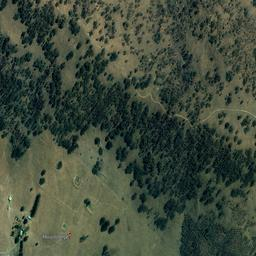
\includegraphics[width=\linewidth]{figures/f1.jpg}
        %\caption{Image from Forest dataset}
    \end{subfigure}
    \hfill
    \begin{subfigure}[t]{0.15\textwidth}
        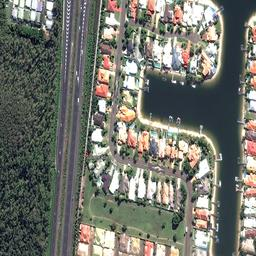
\includegraphics[width=\linewidth]{figures/r3.jpg}
        %\caption{Image from Residence dataset}
    \end{subfigure}
    \hfill
    \begin{subfigure}[t]{0.15\textwidth}
        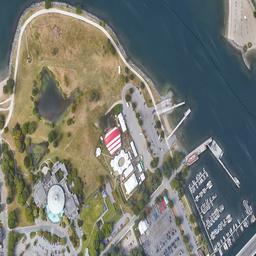
\includegraphics[width=\linewidth]{figures/park1.jpg}
        %\caption{Image from Park dataset}
    \end{subfigure}
    \begin{subfigure}[t]{0.15\textwidth}
        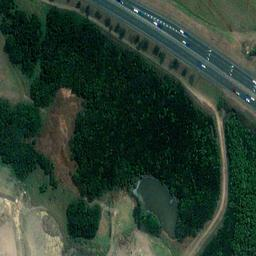
\includegraphics[width=\linewidth]{figures/f2.jpg}
        %\caption{Image from Forest dataset}
    \end{subfigure} 
    \hfill
    \begin{subfigure}[t]{0.15\textwidth}
        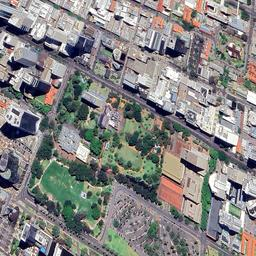
\includegraphics[width=\linewidth]{figures/r2.jpg}
       %\caption{Image from Residence dataset}
    \end{subfigure}
    \hfill
    \begin{subfigure}[t]{0.15\textwidth}
    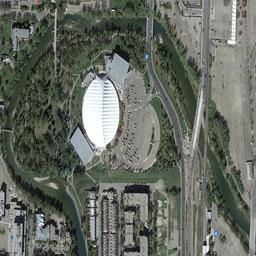
\includegraphics[width=\linewidth]{figures/park2.jpg}
       % \caption{Image from Park dataset}
    \end{subfigure}
    \caption{Sample Images from Categories of Custom Dataset}
    \label{customdatasetimage}
   
\end{figure}
